


\chapter{Receivers} % (fold)
\label{cha:receivers}


\section{Image} % (fold)
\label{sec:image}

\begin{figure}[ht]
	\centering
	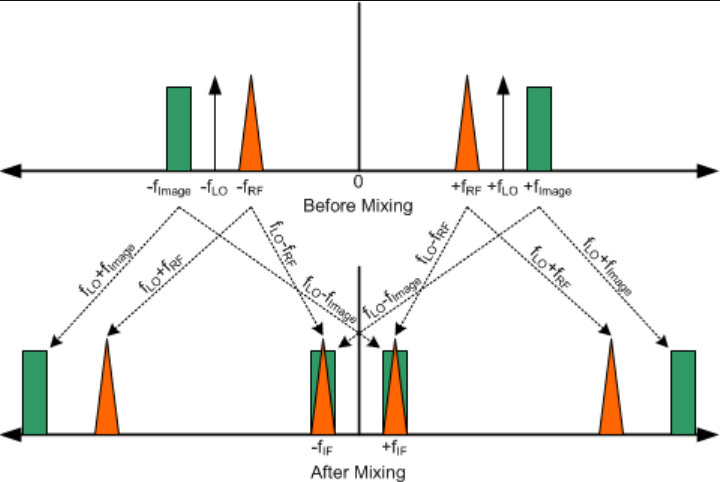
\includegraphics[scale=0.45]{Immagini/image}
	\label{fig:casip}
\end{figure}


The problem of the image rises during the domodulation process when the RF signal is downconverted to an Intermediate Frequncy (IF) because of the mixer by means of the LO downconverts to IF both the RF signal and the Image which any signal at the same opposite distance\footnote{Note that this deistance is by definition IF} from the LO with respect to RF signal.

\subsection*{Example} % (fold)
\label{sub:example}

Let's report an example for clarification\footnote{$1^{st}$ February 2017 exercise 1 question a)}:
\begin{itemize}
	\item $f_{RF}= 12 Ghz$ 
	\item $f_{IF}= 140 Mhz$ 
\end{itemize}

we know that the local oscillator frequency (fLO) is above the signal band.

Find the frequncy of the image is quite simple:


\begin{equation}
	f_{IF}=|f_{RF}-f_{LO}|
\end{equation}

from this we are able to find $f_{LO}$ and then:

\begin{equation}
		f_{IM}=f_{LO}-f_{IF}= f_{RF}-2f_{IF}
\end{equation}

% section image (end)

\section{Cascaded Noise Figure} % (fold)
\label{sec:cascaded_noise_figure}

The evalutation of the Noise figure of cascaded stage could be performed with this formula:

\begin{equation}
	NF_{eq}= NF_1 + \frac{NF_2-1}{G_1} + \frac{NF_3-1}{G_1G_2} 
\end{equation}

% section cascaded_noise_figure (end)


% chapter receivers (end)